% !TEX root = batteryposter.tex

\documentclass[tikz]{standalone}
% !TEX root = batteryposter.tex

\usepackage{mwe}
\usepackage{blindtext}
\usepackage{relsize}
\usetikzlibrary{positioning	}
\usetikzlibrary{arrows.meta}
% Macros
\newcommand{\xo}{\bigotimes}

%%%%%%%%%%%%%%%%%%%%%%%%%%%%%%%%%%%%%%%%%%%%%%%%%%%%%%%%%%%%%%%%%%%%%%%%%%%%%%%%%%%%%%%%
% Poster parameters %%%%%%%%%%%%%%%%%%%%%%%%%%%%%%%%%%%%%%%%%%%%%%%%%%%%%%%%%%%%%%%%%%%%
%%%%%%%%%%%%%%%%%%%%%%%%%%%%%%%%%%%%%%%%%%%%%%%%%%%%%%%%%%%%%%%%%%%%%%%%%%%%%%%%%%%%%%%%

% Colours
\newcommand{\macrocolor}{red}
\newcommand{\microcolor}{blue}
\newcommand{\macrotext}[1]{\color{\macrocolor}#1}
\newcommand{\microtext}[1]{\color{\microcolor}#1}

% Graph box parameters
\newcommand{\FIGWIDTH}{14cm} % figure width
\newcommand{\FIGHEIGHT}{9cm} % figure height
\newcommand{\VERTFIGSEP}{5cm} % vertical separation between figures
\newcommand{\HORFIGSEP}{7cm} % horizontal separation between figures

% Axis box and line style
\tikzstyle{axisbox} = [inner sep=0]
\tikzstyle{axisline} = [
		% {Latex[length=1cm, width=1cm]}-{Latex[length=1cm, width=1cm]},
		-{Latex[length=1cm, width=1cm]},
		ultra thick,
		>=stealth
]

% Model point style
\tikzstyle{modelpoint} = [
		circle,
		fill=black,
		inner sep=0pt,
		minimum size=0.5cm,
		% prefix after command= {\pgfextra{\tikzset{every label/.style={font=\Huge}}}}
]

% Textbox style
\tikzstyle{mybox} = [
		draw=red,
		fill=blue!20,
		very thick,
    rectangle,
		rounded corners,
		inner sep=10pt,
		inner ysep=20pt]
\tikzstyle{fancytitle} = [fill=red, text=white]

%%%%%%%%%%%%%%%%%%%%%%%%%%%%%%%%%%%%%%%%%%%%%%%%%%%%%%%%%%%%%%%%%%%%%%%%%%%%%%%%%%%%%%%%
%%%%%%%%%%%%%%%%%%%%%%%%%%%%%%%%%%%%%%%%%%%%%%%%%%%%%%%%%%%%%%%%%%%%%%%%%%%%%%%%%%%%%%%%


\begin{document}
\begin{tikzpicture}
	% Grid lines (comment out to turn off)
	% \draw[help lines,color=black,xstep=1,ystep=1] (0,0) grid (80,90);
	% \foreach \x in {0,1,...,24} { \node [anchor=north] at (\x,0) {\x}; }
	% \foreach \y in {0,1,...,29} { \node [anchor=east] at (0,\y) {\y}; }

	% Full 3D
	% \node [axisbox, anchor=north west](3d_full) at (0,90) {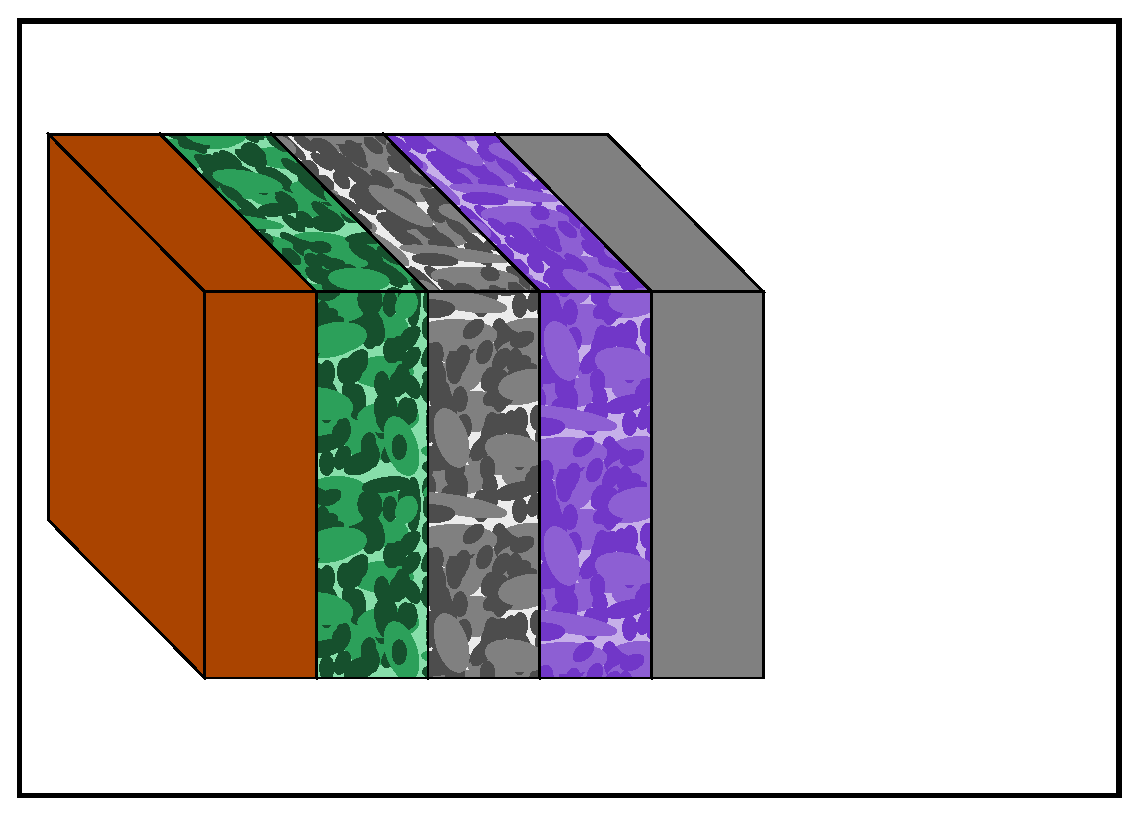
\includegraphics[width=\FIGWIDTH, height=\FIGHEIGHT]{figures/3D_unhomogenised}};

	% % Text
	% \node[textboxtitle,  above right = 0cm and 3cm of 3d_full, anchor=north west]
	% 	(title) {Introduction};
	% \node [textbox, anchor=north west] (box) at (title.south west) {%
	% 	\begin{minipage}{0.75\textwidth}
	% 			\blinditemize[4]
	% 	\end{minipage}
	% };


	% 3 + 3
	% \node [axisbox, below = \VERTFIGSEP of 3d_full, anchor=north](3D_homogenised_micro)
	% 	{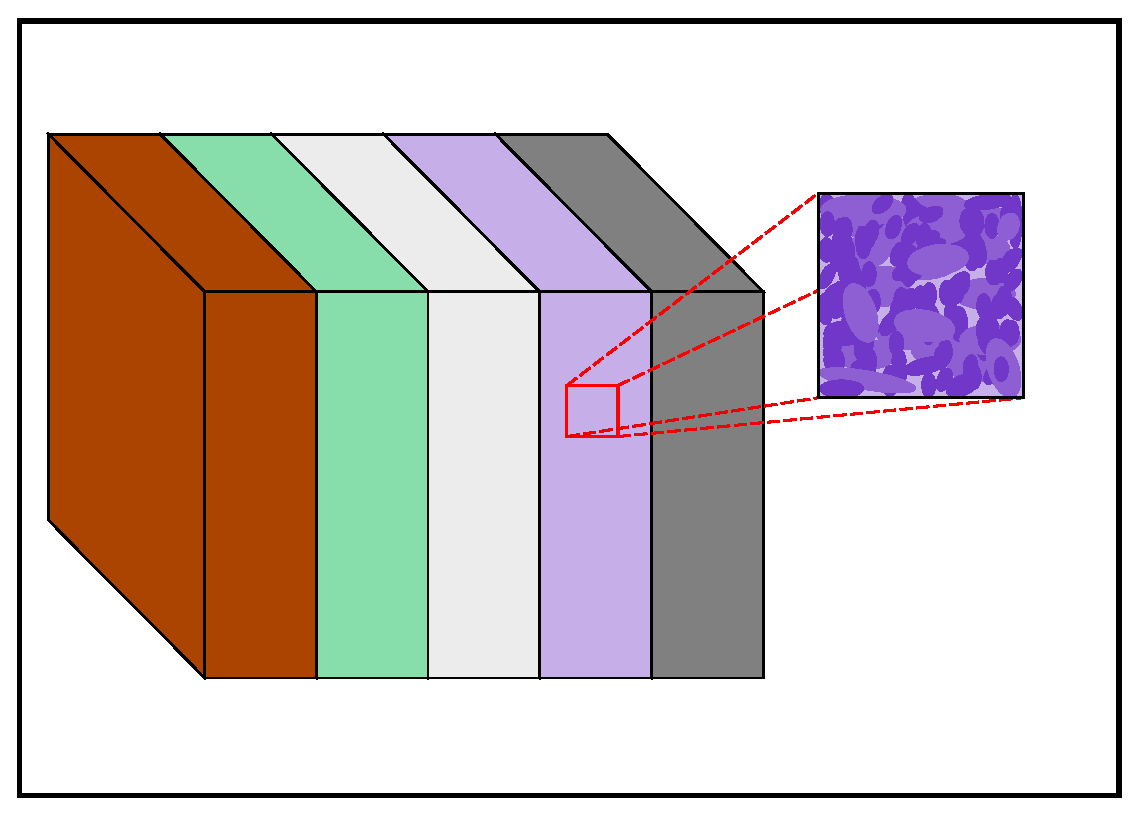
\includegraphics[width=\FIGWIDTH, height=\FIGHEIGHT]{figures/3D_homogenised_micro}};
	\node [axisbox, anchor=north west](3D_homogenised_micro) at (0,70) {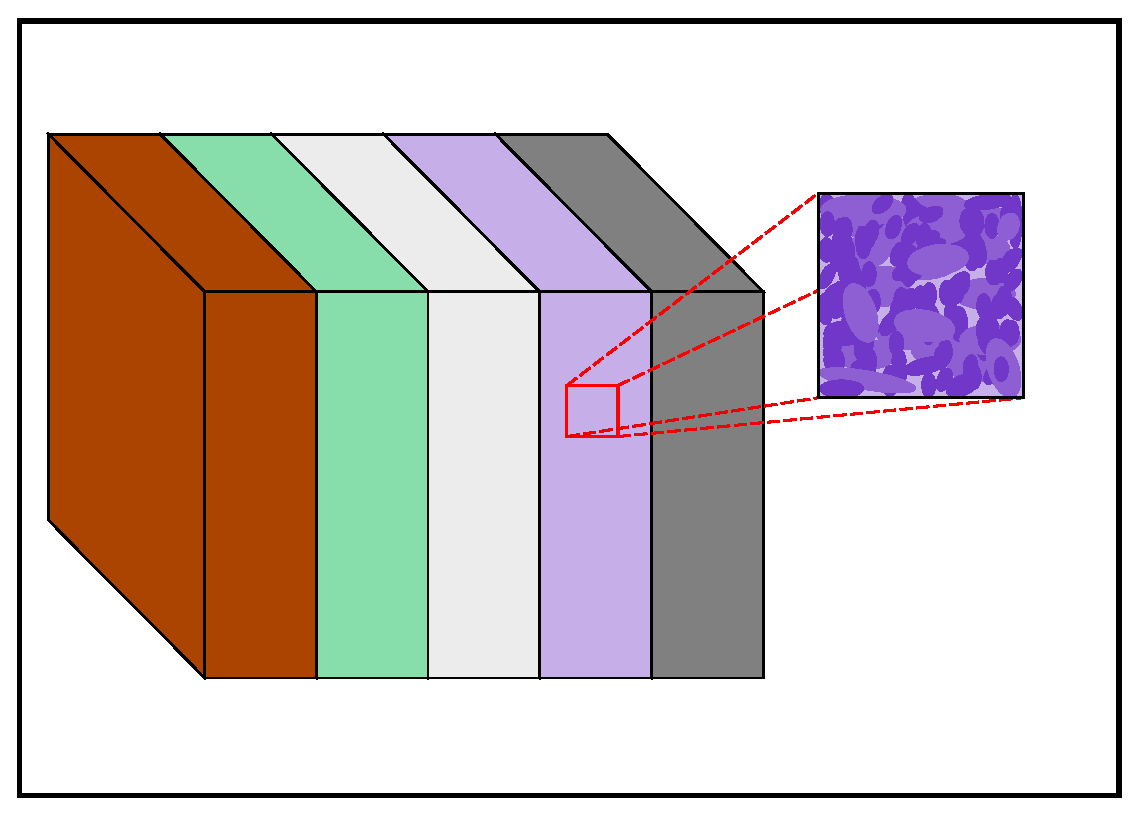
\includegraphics[width=\FIGWIDTH, height=\FIGHEIGHT]{figures/3D_homogenised_micro}};
	\node [dimensions] at (3D_homogenised_micro.north east) {};
	\node [axisbox, anchor=north west](3_plus_3) at (0,70) {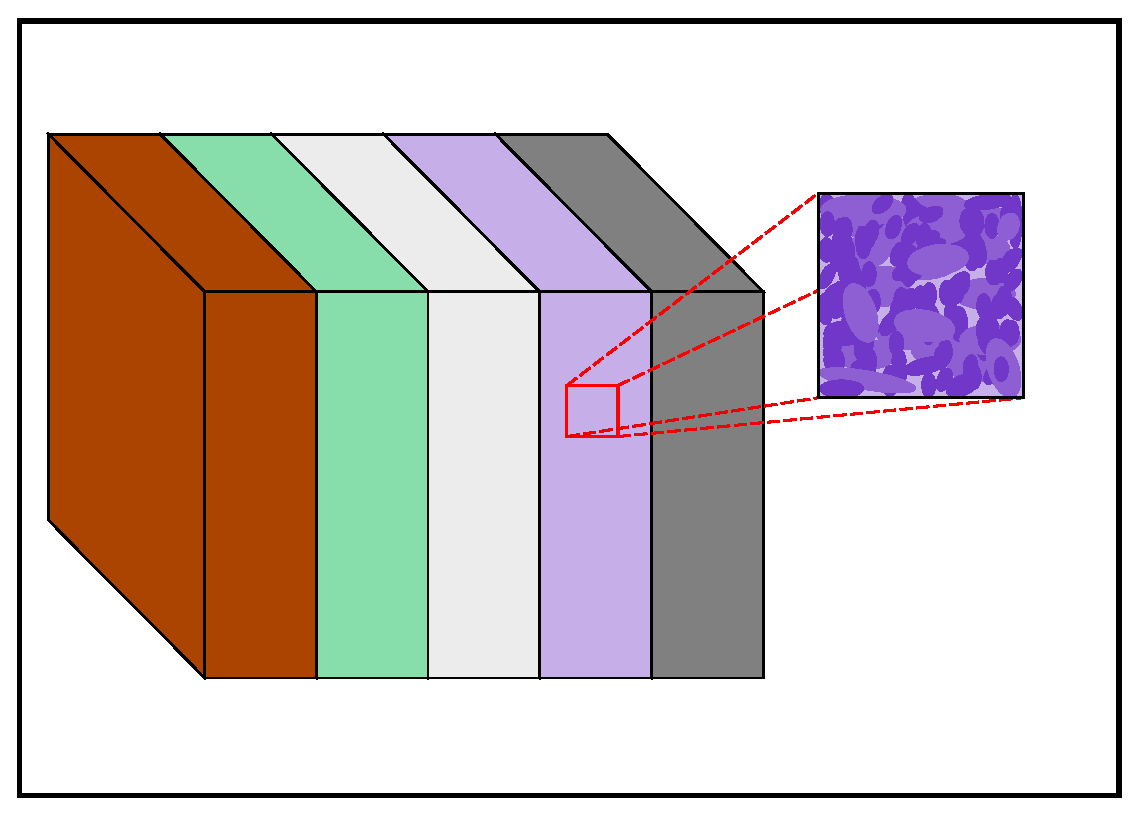
\includegraphics[width=\FIGWIDTH, height=\FIGHEIGHT]{figures/3D_homogenised_micro}};

	%
	% Microscale row and axis
	%
	\node [axisbox, right = \HORFIGSEP of 3D_homogenised_micro, anchor=west]
		(particle_distribution)
		{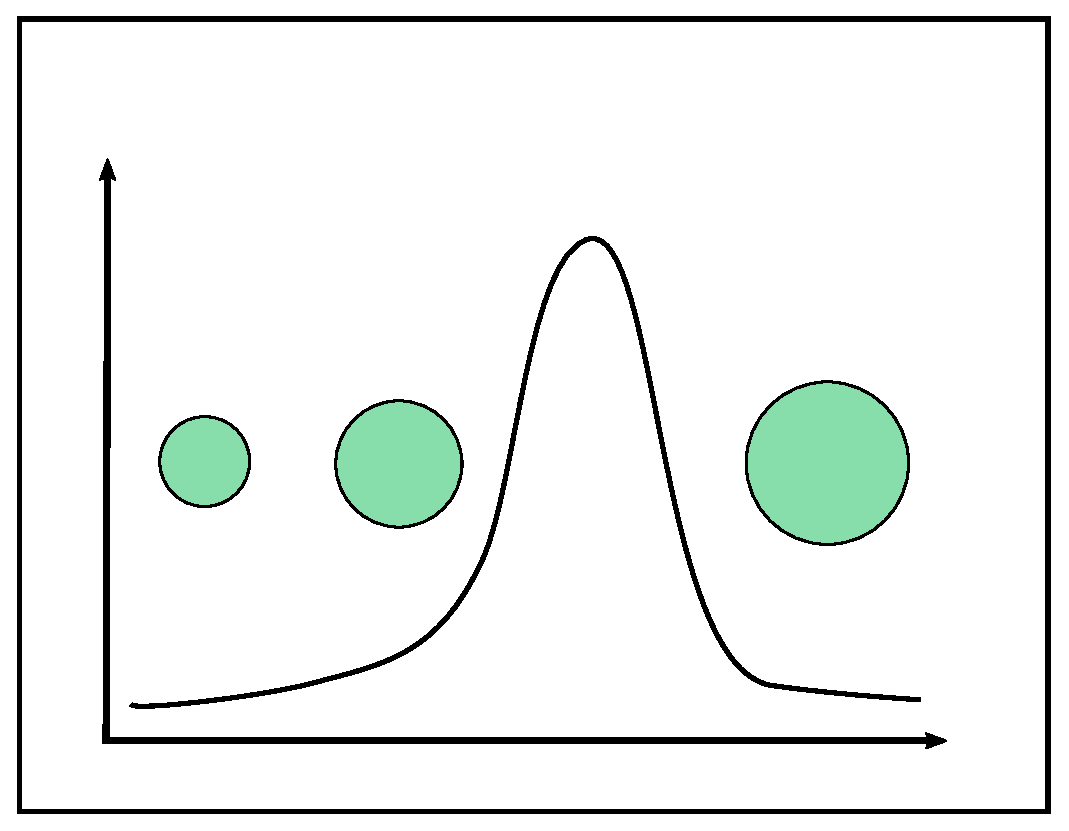
\includegraphics[width=\FIGWIDTH, height=\FIGHEIGHT]
			{figures/particle_distribution}};
	\node [dimensions, microcolor] at (particle_distribution.north east) {$1\xo1$};
	\node [physics] at (particle_distribution.south east) {Spherical \\ particles};
	%
	\node [axisbox, right = \HORFIGSEP of particle_distribution, anchor=west]
		(single_particle)
		{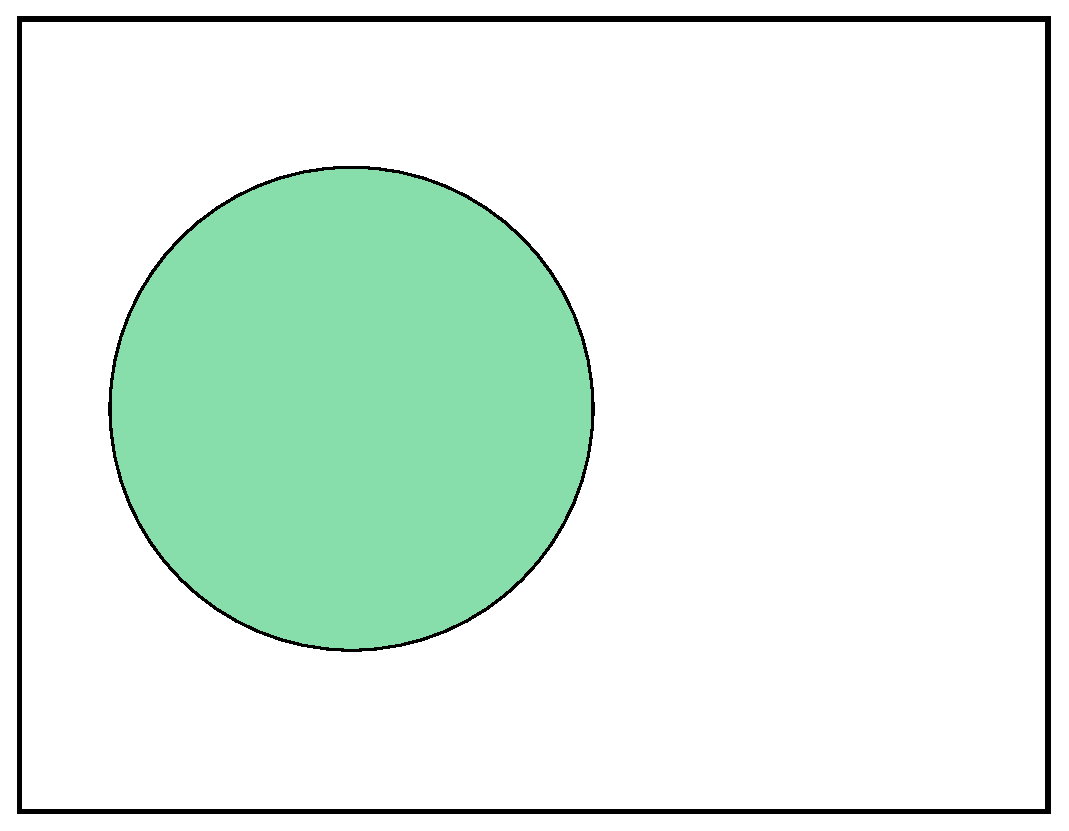
\includegraphics[width=\FIGWIDTH, height=\FIGHEIGHT]{figures/single_particle}};
	\node [dimensions, microcolor] at (single_particle.north east) {$1$};
	\node [physics] at (single_particle.south east) {Narrow \\ particle \\ distribution};
	%
	\node [axisbox, right = \HORFIGSEP of single_particle, anchor=west](0D_micro)
		{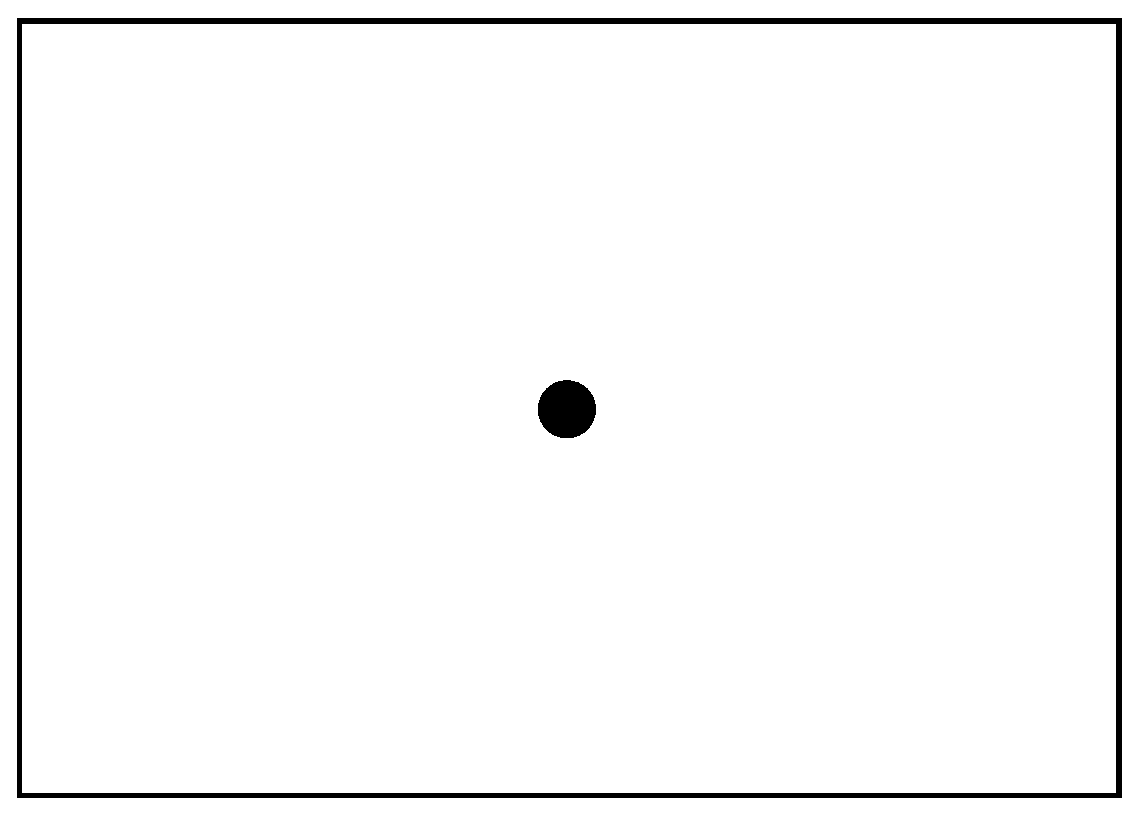
\includegraphics[width=\FIGWIDTH, height=\FIGHEIGHT]{figures/0D}};
	\node [dimensions, microcolor] at (0D_micro.north east) {$0$};
	\node [physics] at (0D_micro.south east) {Fast diffusion \\ in particles};
	% axis
	% \node [below left = 3cm and 0cm of particle_distribution](x_axis_start) {};
	% \node [below right = 3cm and 0cm of 0D_micro](x_axis_end) {};
	\node [below right = 3cm and 2.5cm of 3D_homogenised_micro, anchor=center]
		(axis_origin) {$\xo$};
	\node (x_axis_end) at (axis_origin -| 0D_micro.east) {};
	\draw [axisline, microcolor] (axis_origin) -- (x_axis_end)
		node [above, pos=0, anchor=south west] {Complex}
		node [above, pos=0.5, anchor=south] {\Large \textsc{Microscale}}
		node [above, pos=1, anchor=south east] {Simple};
	%
	% Macroscale column and axis
	%
	\node [axisbox, below = \VERTFIGSEP of 3D_homogenised_micro, anchor=north](2plus1D)
		{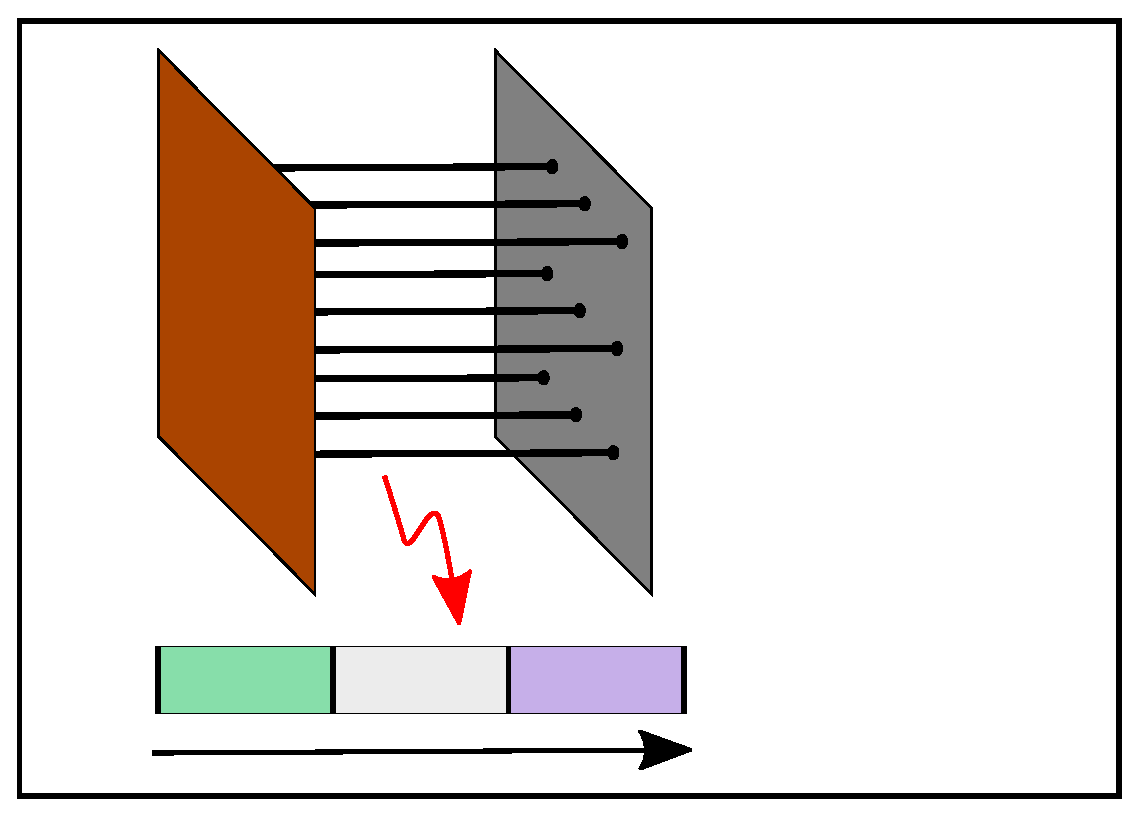
\includegraphics[width=\FIGWIDTH, height=\FIGHEIGHT]{figures/2plus1D}};
	\node [dimensions, macrocolor] at (2plus1D.north east) {$2\xo1$};
	\node [physics] at (2plus1D.south east) {Thin \\ electrodes};
	%
	\node [axisbox, below = \VERTFIGSEP of 2plus1D, anchor=north](2plusbar1D)
		{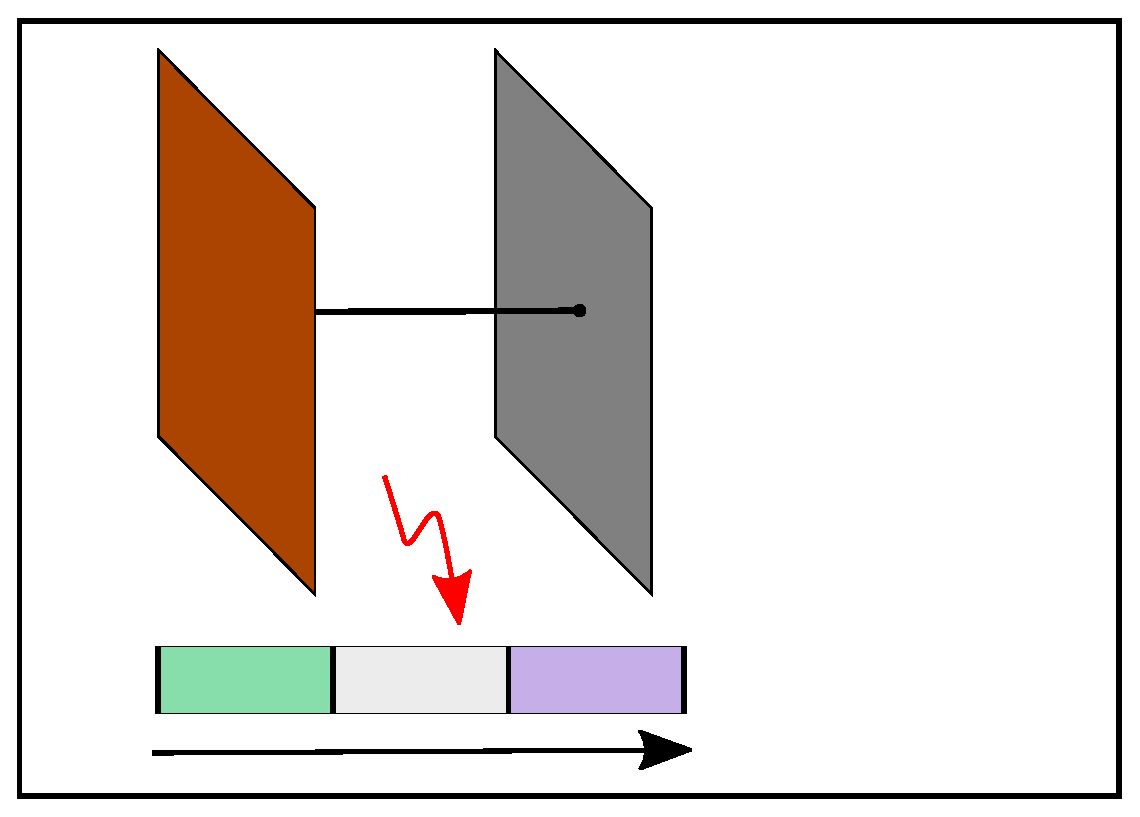
\includegraphics[width=\FIGWIDTH, height=\FIGHEIGHT]{figures/2plusbar1D}};
	\node [dimensions, macrocolor] at (2plusbar1D.north east) {$2\xo\bar{1}$};
	\node [physics] at (2plusbar1D.south east) {Large \\ conductivity};
	%
	\node [axisbox, below = \VERTFIGSEP of 2plusbar1D, anchor=north](0plus1D)
		{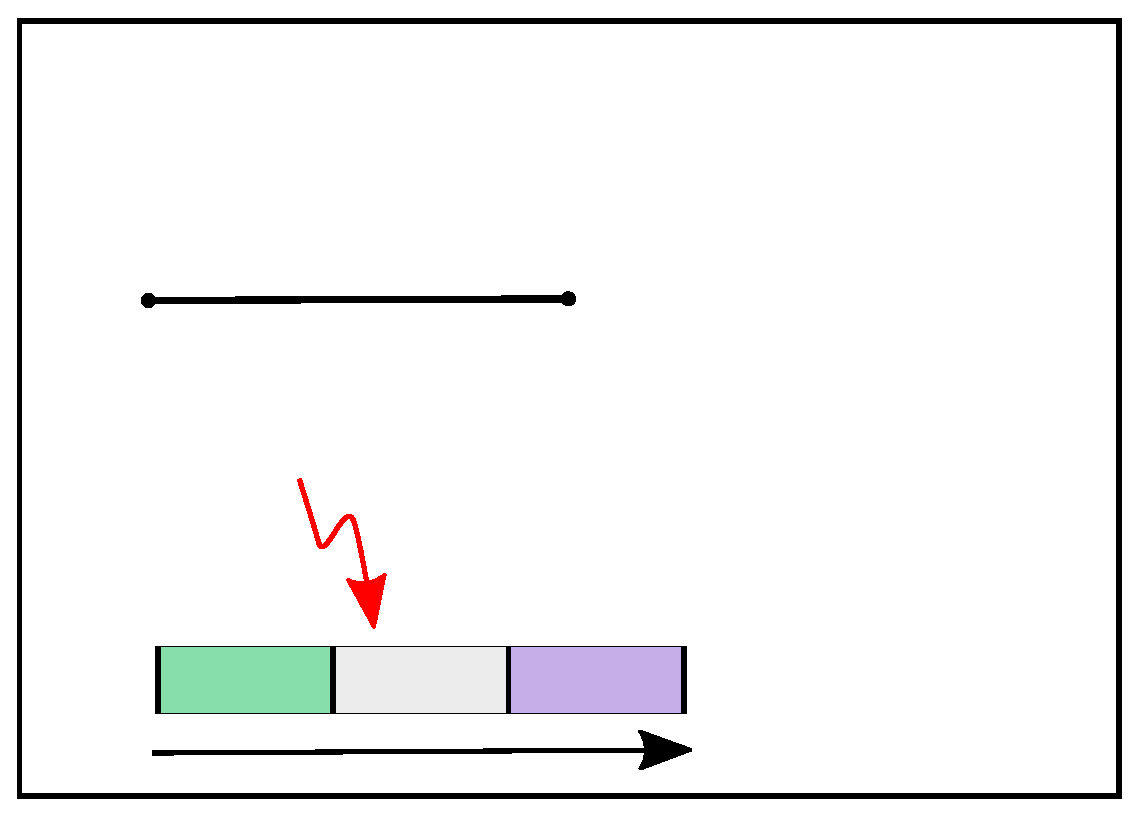
\includegraphics[width=\FIGWIDTH, height=\FIGHEIGHT]{figures/0plus1D}};
	\node [dimensions, macrocolor] at (0plus1D.north east) {$0\xo1$};
	\node [physics] at (0plus1D.south east) {Very large \\ conductivity};
	%
	\node [axisbox, below = \VERTFIGSEP of 0plus1D, anchor=north](0D_macro)
		{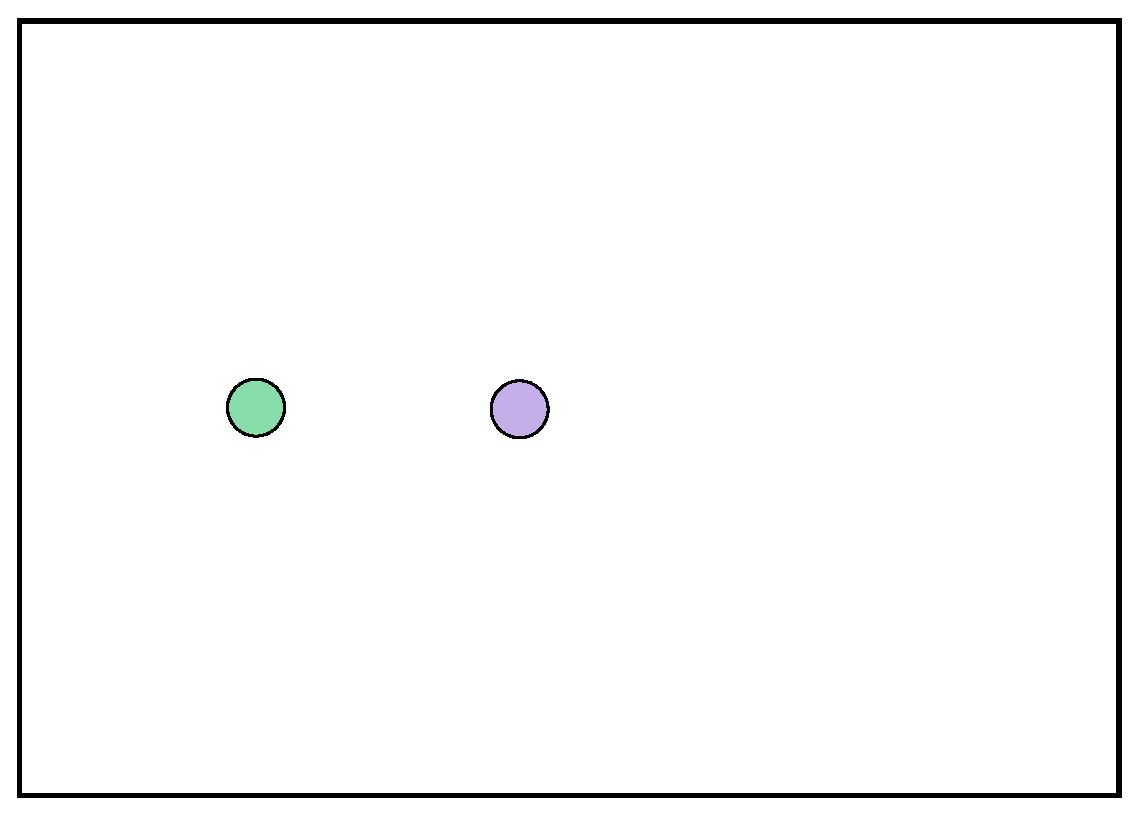
\includegraphics[width=\FIGWIDTH, height=\FIGHEIGHT]{figures/0D_macro}};
	\node [dimensions, macrocolor] at (0D_macro.north east) {$0\xo0$};
	\node [physics] at (0D_macro.south east) {Fast diffusion \\ in electrolyte};
	% axis
	% \node [above right = 0cm and 2.5cm of 2plus1D](y_axis_start) {};
	% \node [below right = 0cm and 2.5cm of 0D_macro](y_axis_end) {};
	\node (y_axis_end) at (0D_macro.south -| axis_origin) {};
	\draw [axisline, macrocolor] (axis_origin) -- (y_axis_end)
		node [left, pos=0, rotate=90, anchor=south east] {Complex}
		node [left, pos=0.5, rotate=90, anchor=south] {\Large \textsc{Macroscale}}
		node [below, rotate=90, anchor=south west] {Simple};

	%%%%%%%%%%%%%%%%%%%%%%%%%%%%%%%%%%%%%%%%%%%%%%%%%%%%%%%%%%%%%%%%%%%%%%%%%%%%%%%%%%%%%%
	% Inner plot %%%%%%%%%%%%%%%%%%%%%%%%%%%%%%%%%%%%%%%%%%%%%%%%%%%%%%%%%%%%%%%%%%%%%%%%%
	%%%%%%%%%%%%%%%%%%%%%%%%%%%%%%%%%%%%%%%%%%%%%%%%%%%%%%%%%%%%%%%%%%%%%%%%%%%%%%%%%%%%%%
	%
	% 2D+1D models
	%
	\node [
		modelpoint,
		label=right:{\includedimensions{$\macrotext{2\xo1}\black{\xo}\microtext{0}$}}
	]
		 (2plus1D_0D) at (2plus1D -| 0D_micro) {};
	\node [
		modelpoint,
		label=right:{
				\includedimensions{$\macrotext{2\xo\bar{1}}\black{\xo}\microtext{1}$ (}
				SPMeCC
				\includedimensions{)}
			}
	]
		(SPMeCC) at (2plusbar1D -| single_particle) {};
	\node [
		modelpoint,
		label=right:{\includedimensions{$\macrotext{2\xo\bar{1}}\black{\xo}\microtext{0}$}}
	]
		(2plusbar1D_0D) at (2plusbar1D -| 0D_micro) {};
	% Results
	\node [axisbox, below left = 5cm and 0cm of particle_distribution, anchor=north west]
		(2D_results) {\includegraphics[width=45cm, height=15cm]{example-image-a}};
	\node [profile_pic] (rob_2D) at (2D_results.south west)
		{\includegraphics[width=\PPWIDTH, height=\PPHEIGHT]{example-image-b}};
	\node [profile_pic] (scott_2D) at (rob_2D.south east)
		{\includegraphics[width=\PPWIDTH, height=\PPHEIGHT]{example-image-b}};
	\node [profile_pic] (tino_2D) at (scott_2D.south east)
		{\includegraphics[width=\PPWIDTH, height=\PPHEIGHT]{example-image-b}};
	% Arrows
	\draw [results_arrow] (2plus1D_0D) -- (2D_results.east);
	\draw [results_arrow] (SPMeCC) -- (2D_results.south);
	\draw [results_arrow] (2plusbar1D_0D) -- (2D_results.south east);

	%
	% DFN, SPMe, SPM
	%
	\node [
		modelpoint,
		label=right:{
			\includedimensions{$\macrotext{0\xo1}\black{\xo}\microtext{1}$ (}
			DFN
			\includedimensions{)}
		}
	]
		(DFN) at (0plus1D -| single_particle) {};
	\node [
		modelpoint,
		label=right:{
			\includedimensions{$\macrotext{0\xo0}\black{\xo}\microtext{1}$ (}
			SPM
			\includedimensions{)}
		}
	]
		(SPM) at (0D_macro -| single_particle) {};
	\node [
		modelpoint,
		label=right:{
			\includedimensions{$\macrotext{0\xo0}\black{\xo}\microtext{1}$ (}
			SPMe
			\includedimensions{)}
		}
	]
		(SPMe) at ($(SPM)!0.5!(DFN)$) {};
	% Results
	\node [axisbox, below left = 2cm and 0cm of 2D_results, anchor=north west]
		(SPM_results) {\includegraphics[width=25cm, height=12cm]{example-image-a}};
	\node [profile_pic] (rob_SPM) at (SPM_results.south west)
		{\includegraphics[width=\PPWIDTH, height=\PPHEIGHT]{example-image-b}};
	\node [profile_pic] (scott_SPM) at (rob_SPM.south east)
		{\includegraphics[width=\PPWIDTH, height=\PPHEIGHT]{example-image-b}};
	% Arrows
	\draw [results_arrow] (DFN) -- (SPM_results.east);
	\draw [results_arrow] (SPMe) -- ($(SPM_results.east)!0.5!(SPM_results.south east)$);
	\draw [results_arrow] (SPM) -- (SPM_results.south east);

	%
	% Distributed particle models
	%
	\node [
		modelpoint,
		label=right:{
				\includedimensions{$\macrotext{0\xo0}\black{\xo}\microtext{1\xo1}$ (}
				DPM
				\includedimensions{)}
			}
	]
		(DPM) at (0D_macro -| particle_distribution) {};
	\node [
		modelpoint,
		label=right:{
			\includedimensions{$\macrotext{0\xo0}\black{\xo}\microtext{1}$ (}
			MPM
			\includedimensions{)}
		}
	]
		(MPM) at ($(SPM)!0.5!(DPM)$) {};
	% Results
	\node [axisbox, below = 2cm of SPM_results, anchor=north] (distributed_results)
		{\includegraphics[width=25cm, height=12cm]{example-image-a}};
	\node [profile_pic] (toby) at (distributed_results.south west)
		{\includegraphics[width=\PPWIDTH, height=\PPHEIGHT]{example-image-b}};
	% Arrows
	\draw [results_arrow] (DPM) -- (distributed_results.south);
	\draw [results_arrow] (MPM)
		-- ($(distributed_results.south)!0.5!(distributed_results.south east)$);
	\draw [results_arrow] (SPM) -- (distributed_results.south east);

	%
	% Fast diffusion models
	%
	\node [
		modelpoint,
		label=right:{\includedimensions{$\macrotext{0\xo1}\black{\xo}\microtext{0}$}}
	]
		(DFNfast) at (0plus1D -| 0D_micro) {};
	\node [
		modelpoint,
		label=right:{\includedimensions{$\macrotext{0\xo0}\black{\xo}\microtext{0}$}}
	]
		(SPMfast) at (0D_macro -| 0D_micro) {};
	\node [
		modelpoint,
		label=right:{
			\includedimensions{$\macrotext{0\xo0}\black{\xo}\microtext{1}$ (}
			\includedimensions{)}
		}
	]
		(SPMefast) at ($(SPMfast)!0.5!(DFNfast)$) {};
\end{tikzpicture}

\end{document}
